\documentclass[11pt,a4paper]{article}
\usepackage[T1]{fontenc}
\usepackage[utf8]{inputenc}
\usepackage[provide=*,italian]{babel}
\usepackage{lmodern}
\usepackage[a4paper,margin=2.4cm]{geometry}
\usepackage{amsmath,amssymb,bm}
\usepackage{booktabs}
\usepackage{graphicx}
\usepackage{float}
\usepackage{xcolor}
\usepackage[most]{tcolorbox}
\usepackage{titlesec}
\usepackage{enumitem}
\usepackage{caption}
\usepackage{array}
\usepackage[hidelinks]{hyperref}
\graphicspath{{../}}

\definecolor{titolo}{RGB}{140,24,36}
\titleformat{\section}{\Large\bfseries\color{titolo}}{\thesection.}{0.6em}{}
\titleformat{\subsection}{\large\bfseries}{}{0em}{}
\titlespacing*{\section}{0pt}{1.6em}{0.9em}
\titlespacing*{\subsection}{0pt}{1.2em}{0.6em}
\captionsetup{font=small,labelfont=bf}
\setlist{itemsep=0.25em}
\setlength{\parindent}{0pt}
\setlength{\parskip}{0.55em}

\newtcolorbox{nota}[1][]{colback=titolo!5,colframe=titolo!55,boxrule=0.5pt,arc=2pt,left=8pt,right=8pt,top=6pt,bottom=6pt,#1}

\begin{document}

{\color{titolo}\LARGE\bfseries Un modello ARIMA per i Treasury a 10 anni}\\[0.3em]
{\large Serie GS10 mensile, 2000-01 -- 2026-10: stazionarietà, identificazione, stima, diagnostica e previsione}
\vspace{0.4em}\hrule\vspace{1.2em}

\textbf{In sintesi.} Il livello del rendimento ha una radice unitaria; le sue variazioni mensili sono stazionarie, senza drift, e seguono un MA(1). Il modello scelto è un \textbf{ARIMA(0,\,1,\,1) senza costante} con $\hat\theta = 0{,}305$. La componente MA ha una spiegazione precisa: ogni dato è la media dei valori giornalieri del mese, e la media di un random walk produce proprio un MA(1) con $\theta \approx 0{,}27$. Il modello supera tutti i controlli sui residui tranne la normalità (code spesse) e fuori campione riduce l'errore quadratico medio del random walk di circa il 6\%.

%=====================================================================
\section{Dati e scelta della trasformazione}

\textbf{La serie.} GS10 (FRED) è il rendimento dei titoli di Stato USA a 10 anni a scadenza costante, in punti percentuali. I dati sono mensili, da 2000-01 a 2026-10 ($T = 322$ osservazioni), e ogni valore è la \textbf{media dei giorni lavorativi} del mese. Il tasso parte da 6{,}66\% nel 2000, tocca il minimo di 0{,}62\% a luglio 2020 e chiude a 5{,}13\%.

Notazione: $y_t$ è il livello del rendimento (in \%), $\Delta y_t = y_t - y_{t-1}$ la sua variazione mensile (in punti percentuali).

\begin{figure}[H]
\centering
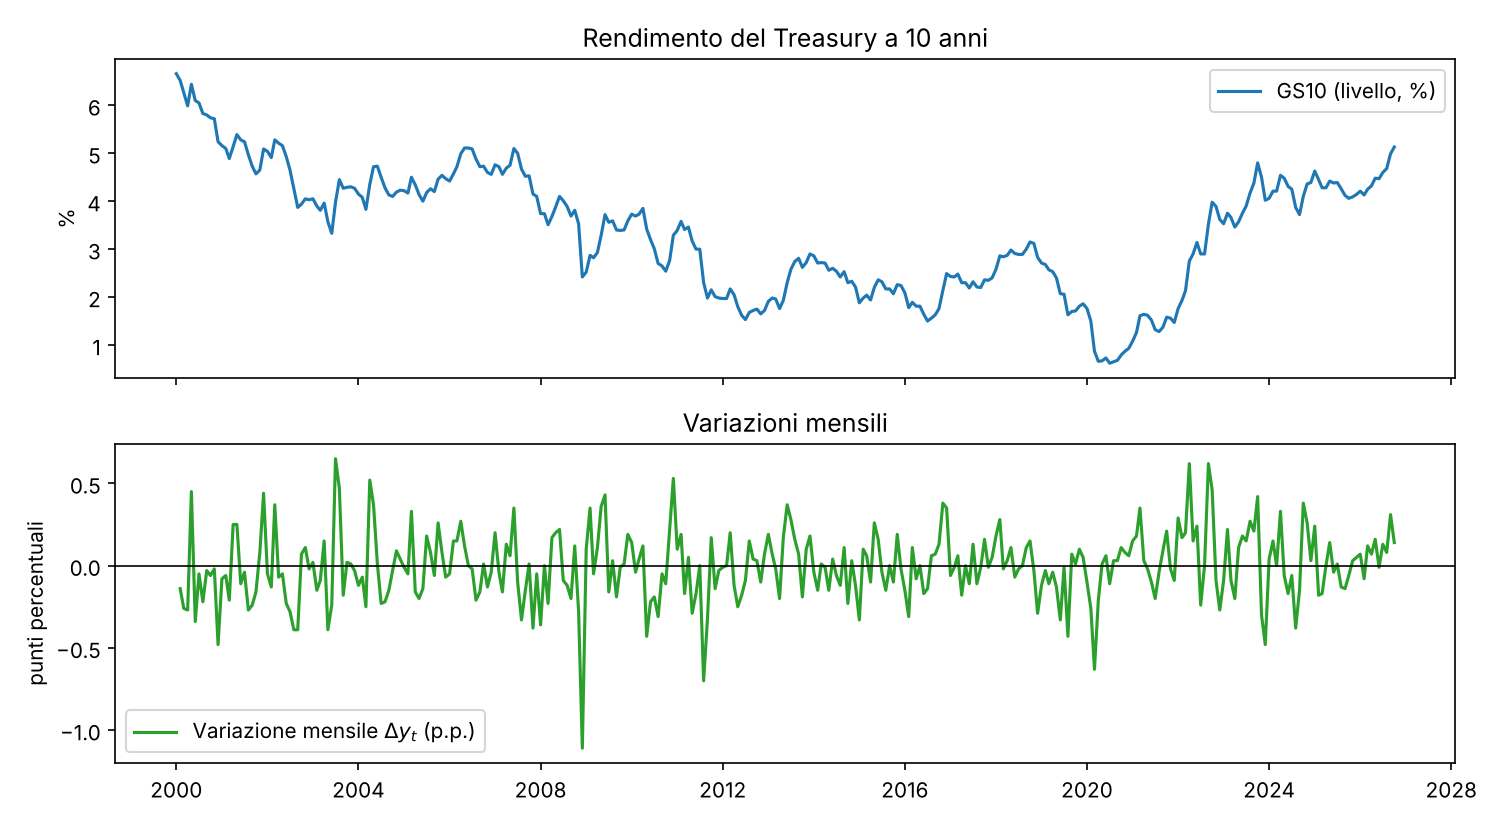
\includegraphics[width=0.92\textwidth]{figures/serie.png}
\caption{Livello di GS10 e variazioni mensili.}
\end{figure}

\subsection{Livelli o logaritmi?}

\begin{nota}
\textbf{GS10 non è un prezzo.} È un tasso d'interesse. La differenza dei logaritmi $\Delta\log y_t$ non è un rendimento ma la variazione \emph{percentuale del tasso}: con il tasso allo 0,62\% una variazione di 0,1 punti vale il 16\%, con il tasso al 5\% vale il 2\%.
\end{nota}

Il corso non tratta modelli per la varianza che cambia nel tempo (GARCH), quindi conviene lavorare con la trasformazione che ha la \textbf{varianza più stabile}. La tabella confronta le due possibili serie di differenze in quattro sottoperiodi.

\begin{table}[H]
\centering
\begin{tabular}{lccc}
\toprule
Periodo & Livello medio (\%) & sd di $\Delta y_t$ (p.p.) & sd di $\Delta\log y_t$ \\
\midrule
2000--2007 & $4{,}69$ & $0{,}218$ & $0{,}049$ \\
2008--2014 & $2{,}80$ & $0{,}234$ & $0{,}085$ \\
2015--2021 & $1{,}96$ & $0{,}168$ & $0{,}108$ \\
2022--2026 & $3{,}97$ & $0{,}223$ & $0{,}067$ \\
\midrule
Rapporto max/min & & $1{,}40$ & $2{,}23$ \\
\bottomrule
\end{tabular}
\caption{Deviazione standard delle variazioni per sottoperiodo.}
\end{table}

In punti percentuali la deviazione standard resta tra circa 0,17 e 0,23; in logaritmi più che raddoppia negli anni dei tassi vicini allo zero (figura~\ref{fig:var}). \textbf{Il modello è quindi costruito sui livelli.}

\begin{figure}[H]
\centering
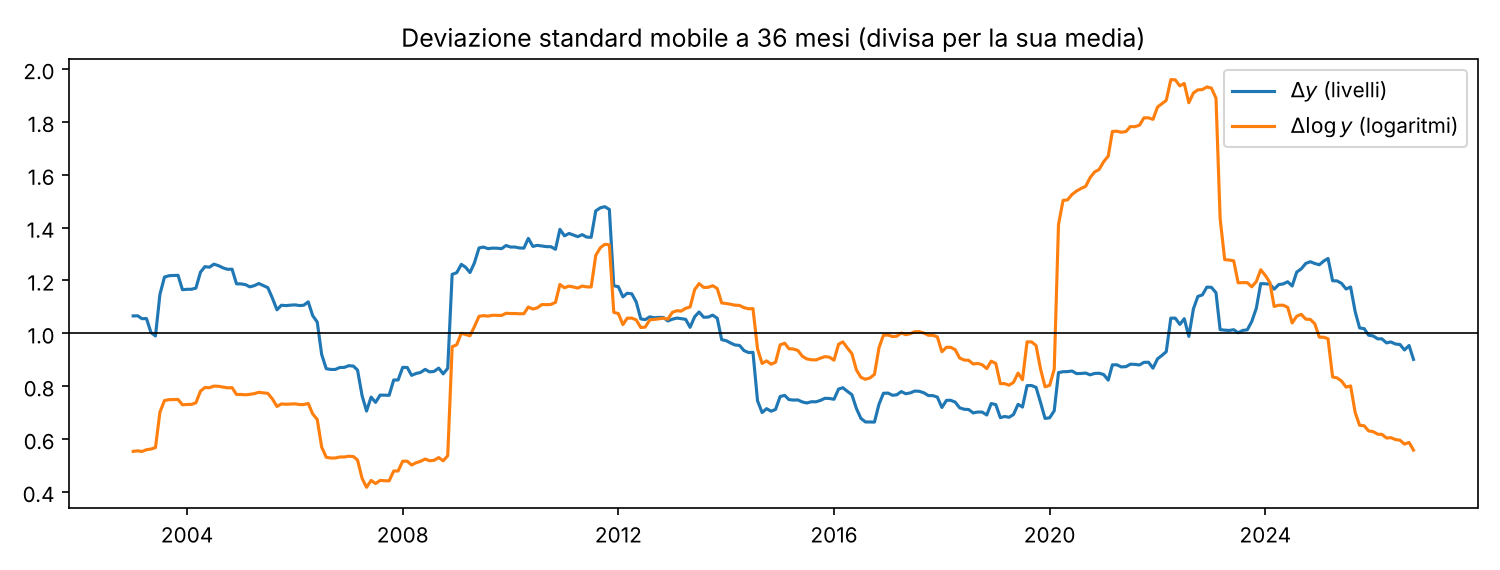
\includegraphics[width=0.85\textwidth]{figures/varianza_mobile.png}
\caption{Deviazione standard mobile a 36 mesi, divisa per la sua media: i logaritmi amplificano la variabilità quando i tassi sono bassi.}
\label{fig:var}
\end{figure}

\textbf{Distribuzione.} Le variazioni mensili hanno media $-0{,}0048$, deviazione standard $0{,}213$, asimmetria $-0{,}22$ e curtosi $5{,}45$: code più spesse di una normale (mesi estremi come fine 2008 e il 2022).

%=====================================================================
\section{Stazionarietà: scelta di $d$}

\textbf{Perché due test.} ADF e KPSS hanno le ipotesi invertite e ciascuno conserva $H_0$ finché i dati non la smentiscono:
\begin{itemize}
\item \textbf{ADF}: $H_0$ radice unitaria. Regressione $\Delta y_t = \alpha\,(+\beta t) + \delta\,y_{t-1} + \sum_j \gamma_j \Delta y_{t-j} + e_t$, statistica $\tau = \hat\delta/SE(\hat\delta)$, si rifiuta nella \textbf{coda sinistra}. I ritardi sono scelti con l'AIC su un campione comune; i valori critici sono quelli di MacKinnon per il $T$ effettivo.
\item \textbf{KPSS}: $H_0$ stazionarietà. Statistica $\eta = \sum_t S_t^2 / (T^2\hat\sigma^2_{LR})$, con $S_t$ somme parziali dei residui; si rifiuta nella \textbf{coda destra}. $L = \lfloor 4(T/100)^{1/4}\rfloor$ ritardi per $\hat\sigma^2_{LR}$.
\end{itemize}

\textbf{Quale versione.} Sui livelli si usano sia \texttt{'c'} (media costante) sia \texttt{'ct'} (trend deterministico), perché la serie scende per vent'anni e poi risale. Sulle differenze solo \texttt{'c'}: un trend lineare nei livelli diventerebbe una costante nelle differenze.

\begin{table}[H]
\centering
\small
\begin{tabular}{llcccl|ccl}
\toprule
Serie & Vers. & ADF $\tau$ & lag & crit.\ 5\% & ADF dice & KPSS $\eta$ & crit.\ 5\% & KPSS dice \\
\midrule
$y_t$ & \texttt{'c'} & $-2{,}19$ & 2 & $-2{,}87$ & radice unitaria & $2{,}073$ & $0{,}463$ & non stazionaria \\
$y_t$ & \texttt{'ct'} & $-1{,}45$ & 2 & $-3{,}42$ & radice unitaria & $0{,}862$ & $0{,}146$ & non stazionaria \\
$\Delta y_t$ & \texttt{'c'} & $-12{,}36$ & 1 & $-2{,}87$ & stazionaria & $0{,}420$ & $0{,}463$ & stazionaria \\
\bottomrule
\end{tabular}
\caption{Test di stazionarietà. ADF: rifiuto se $\tau <$ critico. KPSS: rifiuto se $\eta >$ critico.}
\end{table}

I due test concordano: \textbf{il livello ha una radice unitaria, le variazioni sono stazionarie}. Quindi $d = 1$, e una seconda differenza non serve.

\subsection{Drift}

Con $d = 1$ la costante del modello è il drift, la variazione media mensile. Il t-test sulla media di $\Delta y_t$ con errori standard di Newey-West (necessari perché $\Delta y_t$ è autocorrelata) dà $t = -0{,}36$, p-value $0{,}72$: \textbf{drift non significativo}, quindi il modello non ha costante.

\begin{nota}
\textbf{Perché il trend non si testa sui livelli.} La regressione $y_t = a + bt + u_t$ darebbe $t = -3{,}41$, apparentemente significativo. Ma con una radice unitaria quel $t$ non segue la normale ed è gonfiato (regressione spuria). Per questo, dopo un ADF che non rifiuta, il drift si testa sulle differenze.
\end{nota}

%=====================================================================
\section{C'è qualcosa da modellare?}

Se $\Delta y_t$ fosse rumore bianco il modello migliore sarebbe il random walk, $\hat y_{T+1} = y_T$. Il test di \textbf{Ljung-Box},
\[
Q = T(T+2)\sum_{k=1}^{m}\frac{\hat\rho_k^2}{T-k} \sim \chi^2_{m},
\]
con $m$ gradi di libertà perché non è stato stimato nessun parametro ARMA, rifiuta:

\begin{table}[H]
\centering
\begin{tabular}{cccccl}
\toprule
$m$ & g.d.l. & $Q$ & crit.\ 5\% & p-value & Esito \\
\midrule
6 & 6 & $22{,}76$ & $12{,}59$ & $0{,}0009$ & autocorrelazione \\
12 & 12 & $27{,}45$ & $21{,}03$ & $0{,}0067$ & autocorrelazione \\
\bottomrule
\end{tabular}
\caption{Ljung-Box sulle variazioni mensili.}
\end{table}

Le variazioni sono autocorrelate. Il Durbin-Watson dei residui del random walk (che sono proprio le $\Delta y_t$) vale $1{,}514$, cioè $\hat\rho_1 \approx 1 - d/2 = 0{,}24$.

%=====================================================================
\section{Identificazione: ACF e PACF}

\begin{itemize}
\item \textbf{ACF} con bande di \textbf{Bartlett}: al ritardo $k$ la banda è $\pm1{,}96\sqrt{(1 + 2\sum_{j<k}\hat\rho_j^2)/T}$, il test di $H_0$: MA($k-1$).
\item \textbf{PACF} con banda $\pm 1{,}96/\sqrt T = \pm0{,}109$, il test di $H_0$: AR($k-1$).
\item Il suggerimento è il \textbf{primo ritardo non significativo meno uno}: è lì che la funzione "si interrompe".
\end{itemize}

\begin{figure}[H]
\centering
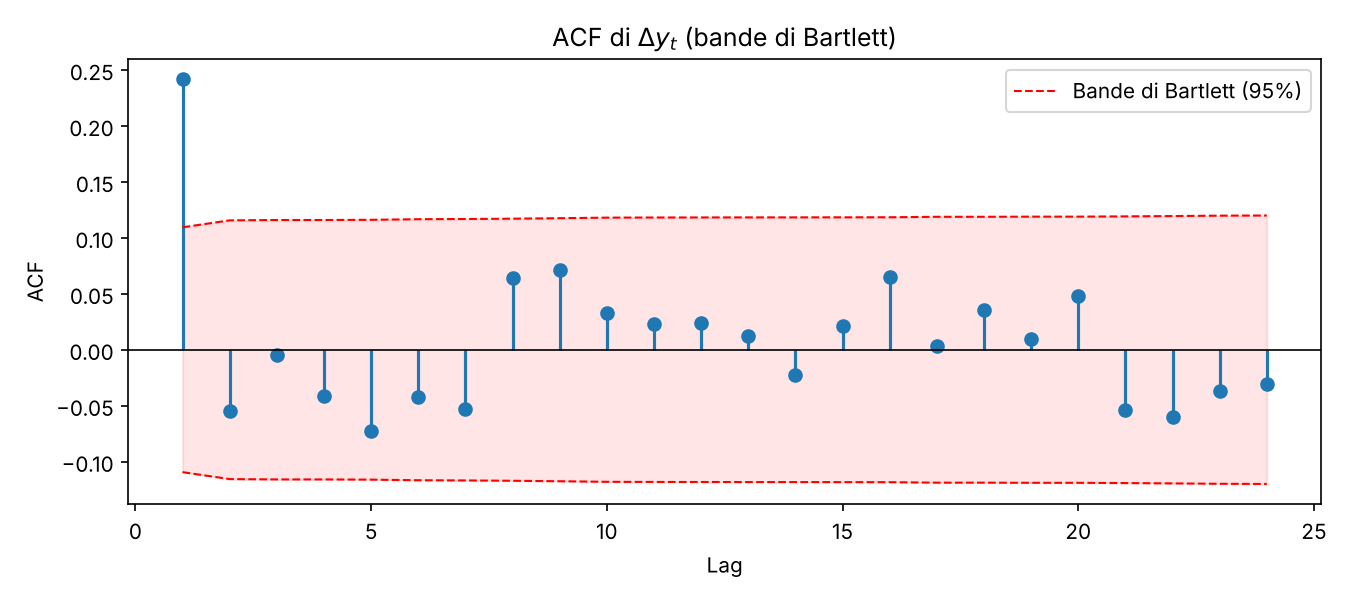
\includegraphics[width=0.49\textwidth]{figures/acf_dy.png}\hfill
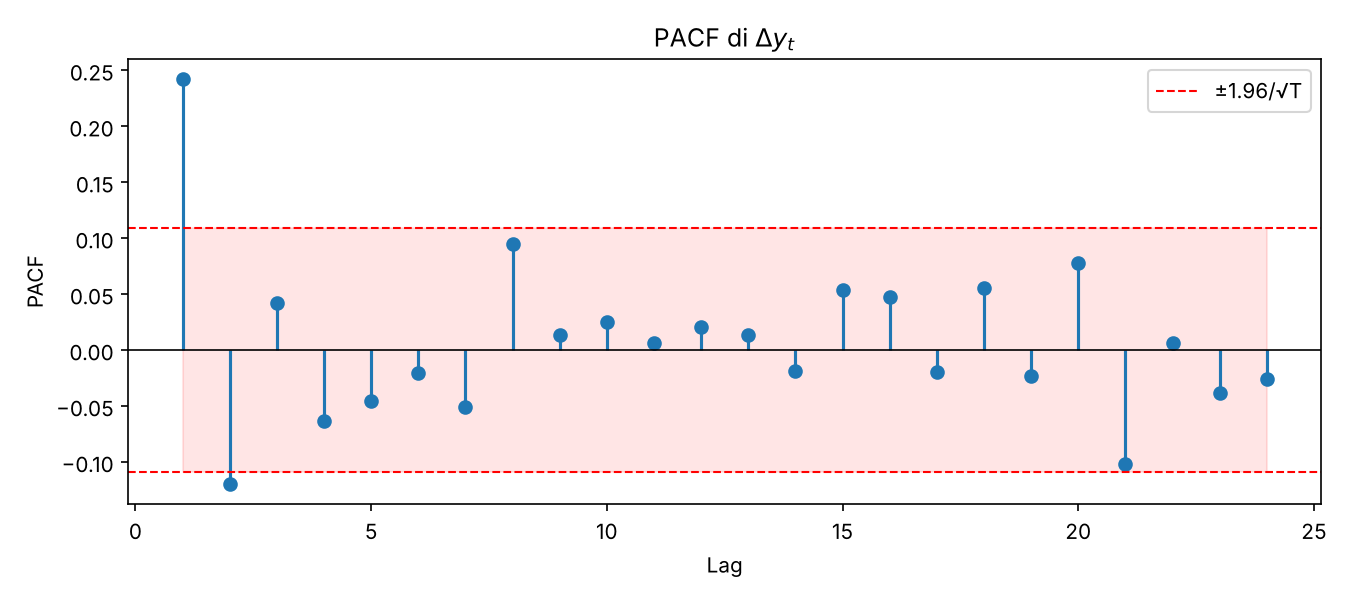
\includegraphics[width=0.49\textwidth]{figures/pacf_dy.png}
\caption{ACF (bande di Bartlett) e PACF di $\Delta y_t$.}
\end{figure}

\begin{table}[H]
\centering
\begin{tabular}{lcccccc}
\toprule
Ritardo & 1 & 2 & 3 & 4 & 5 & 6 \\
\midrule
ACF & $0{,}242$ & $-0{,}055$ & $-0{,}004$ & $-0{,}042$ & $-0{,}072$ & $-0{,}042$ \\
PACF & $0{,}242$ & $-0{,}120$ & $0{,}042$ & $-0{,}064$ & $-0{,}045$ & $-0{,}021$ \\
\bottomrule
\end{tabular}
\end{table}

L'ACF ha una sola barra significativa, al ritardo 1, e poi si interrompe: la firma di un \textbf{MA(1)}. La PACF decresce con segno alterno (0,24 e poi $-0{,}12$), come in un MA(1) con $\theta > 0$; presa alla lettera suggerisce anche un AR(2). Inoltre $\hat\rho_1 > 0$: la differenza non è eccessiva (con una differenza di troppo $\hat\rho_1$ sarebbe vicino a $-0{,}5$).

\begin{nota}
\textbf{Perché non "l'ultimo ritardo significativo".} Su 20 ritardi, ciascuno con il 5\% di probabilità di uscire dalle bande per caso, la probabilità che almeno uno esca è $1 - 0{,}95^{20} \approx 64\%$. La regola della versione precedente aveva preso una barra casuale al ritardo 15 e portato a un ARMA(15,\,1).
\end{nota}

\subsection{Da dove viene l'MA(1): la media mensile}

Supponiamo che il tasso \emph{giornaliero} sia un random walk, $x_s = x_{s-1} + u_s$ con shock indipendenti di varianza $\sigma_u^2$, e che il dato mensile sia la media degli $M$ giorni del mese, $A_k = \frac1M\sum_{i=1}^M x_{(k-1)M+i}$.

\textbf{Peso di ogni shock.} Lo shock del giorno $i$ del mese $k$ sposta tutti i valori successivi. Nella media del mese $k$ entra in $M - i + 1$ giorni su $M$; nella media del mese $k+1$ in tutti. Nelle variazioni $\Delta A_k = A_k - A_{k-1}$ e $\Delta A_{k+1} = A_{k+1} - A_k$ pesa quindi
\[
\text{in } \Delta A_k:\ \frac{M-i+1}{M}, \qquad \text{in } \Delta A_{k+1}:\ 1 - \frac{M-i+1}{M} = \frac{i-1}{M}.
\]

\textbf{Covarianza.} $\Delta A_k$ e $\Delta A_{k+1}$ condividono solo gli shock del mese $k$. Con $j = i - 1$:
\[
Cov(\Delta A_k, \Delta A_{k+1}) = \frac{\sigma_u^2}{M^2}\sum_{j=0}^{M-1} (M - j)\,j = \frac{\sigma_u^2}{M^2}\cdot\frac{M(M^2-1)}{6}.
\]
\textbf{Varianza.} $\Delta A_k$ contiene gli shock del mese $k-1$ con pesi $j/M$ e quelli del mese $k$ con pesi $(M-j)/M$:
\[
Var(\Delta A_k) = \frac{\sigma_u^2}{M^2}\left[\sum_{j=0}^{M-1} j^2 + \sum_{j=1}^{M} j^2\right] = \frac{\sigma_u^2}{M^2}\cdot\frac{M(4M^2+2)}{6}.
\]
\textbf{Autocorrelazione.}
\[
\rho_1 = \frac{M^2 - 1}{2(2M^2+1)} \;\xrightarrow{M\to\infty}\; \frac14, \qquad \rho_k = 0 \ \text{per } k \ge 2,
\]
perché due variazioni distanti due mesi non hanno shock in comune. Con $M = 21$ giorni lavorativi $\rho_1 = 0{,}249$. Un'autocorrelazione solo al primo ritardo è esattamente un MA(1), e il suo $\theta$ risolve
\[
\frac{\theta}{1+\theta^2} = \frac14 \;\Rightarrow\; \theta^2 - 4\theta + 1 = 0 \;\Rightarrow\; \theta = 2 - \sqrt3 \approx 0{,}268.
\]
L'autocorrelazione osservata ($\hat\rho_1 = 0{,}242$) è molto vicina a $1/4$ (Working, 1960).

%=====================================================================
\section{Selezione dell'ordine: AIC e BIC}

Tutti gli ARMA($p$, $q$) con $p, q \le 3$ su $\Delta y_t$ senza costante, più l'ARMA(15,\,1) della versione precedente, confrontati \textbf{sulle stesse osservazioni} (scartate le prime 16):
\[
AIC = \log\frac{RSS}{n} + \frac{2k}{n}, \qquad BIC = \log\frac{RSS}{n} + \frac{k\log n}{n}.
\]

\begin{table}[H]
\centering
\begin{tabular}{lccc}
\toprule
Modello per $\Delta y_t$ & $k$ & AIC & BIC \\
\midrule
ARMA(0, 1) & 1 & $-3{,}1951$ & $-3{,}1829$ \\
ARMA(0, 2) & 2 & $-3{,}1942$ & $-3{,}1698$ \\
ARMA(1, 1) & 2 & $-3{,}1883$ & $-3{,}1639$ \\
ARMA(2, 0) & 2 & $-3{,}1879$ & $-3{,}1635$ \\
ARMA(1, 0) & 1 & $-3{,}1745$ & $-3{,}1623$ \\
ARMA(1, 2) & 3 & $-3{,}1884$ & $-3{,}1518$ \\
\midrule
ARMA(15, 1) & 16 & $-3{,}1201$ & $-2{,}9250$ \\
\bottomrule
\end{tabular}
\caption{I sei modelli con il BIC più basso e l'ARMA(15,\,1) (17° su 17).}
\end{table}

L'\textbf{MA(1)} ha sia il BIC sia l'AIC più bassi. I modelli vicini aggiungono un parametro senza migliorare abbastanza l'adattamento; l'ARMA(15,\,1) usa 16 parametri per descrivere quello che un solo $\theta$ descrive già. Modello scelto:
\[
\boxed{\Delta y_t = \varepsilon_t + \theta\,\varepsilon_{t-1}} \qquad \text{cioè ARIMA(0,\,1,\,1) senza costante.}
\]

%=====================================================================
\section{Stima e controllo del coefficiente}

\textbf{Hannan-Rissanen.} Gli shock $\varepsilon_{t-1}$ non si osservano, quindi non si può stimare $\theta$ con un OLS diretto. Si procede in due passi:
\begin{enumerate}
\item si stima con OLS un AR lungo, di ordine $\lfloor(\log T)^2\rfloor$, e i suoi residui $\tilde\varepsilon_t$ fanno da stima degli shock;
\item si stima con OLS $\Delta y_t = \theta\,\tilde\varepsilon_{t-1} + e_t$; l'errore standard viene da $\hat\sigma^2(X'X)^{-1}$.
\end{enumerate}
Gli shock del modello finale si ricostruiscono poi in modo ricorsivo: $\hat\varepsilon_t = \Delta y_t - \hat\theta\,\hat\varepsilon_{t-1}$.

\begin{table}[H]
\centering
\begin{tabular}{lc}
\toprule
$\hat\theta$ & $0{,}3053$ \\
$SE(\hat\theta)$ & $0{,}0621$ \\
$t$ & $4{,}92$ \quad (p-value $< 10^{-5}$) \\
$\hat\sigma$ (p.p.) & $0{,}2054$ \\
Radice di $1 + \hat\theta z$ & $|z| = 3{,}28$ \\
\midrule
$H_0$: $\theta = 2 - \sqrt3 = 0{,}2679$ & $z = 0{,}60$, p-value $0{,}55$ \\
\bottomrule
\end{tabular}
\caption{Stima dell'ARIMA(0,\,1,\,1).}
\end{table}

\begin{itemize}
\item $\hat\theta$ è molto significativo: la componente MA è reale.
\item La radice MA è fuori dal cerchio unitario: il modello è \textbf{invertibile}, quindi gli shock passati si ricostruiscono dai dati e la rappresentazione è unica.
\item $H_0$: $\theta = 2-\sqrt3$ \textbf{non è rifiutata}: la dinamica stimata è compatibile con quella prodotta dalla sola media mensile di un random walk giornaliero.
\end{itemize}

%=====================================================================
\section{Diagnostica dei residui}

Se il modello è corretto, i residui sono rumore bianco. Il Ljung-Box sui residui ha $m - p - q = m - 1$ gradi di libertà: il parametro stimato rende i residui "più bianchi" del caso e ne consuma uno.

\begin{table}[H]
\centering
\begin{tabular}{cccccl}
\toprule
$m$ & g.d.l. & $Q$ & crit.\ 5\% & p-value & Esito \\
\midrule
6 & 5 & $2{,}98$ & $11{,}07$ & $0{,}704$ & rumore bianco \\
12 & 11 & $7{,}07$ & $19{,}68$ & $0{,}793$ & rumore bianco \\
24 & 23 & $13{,}95$ & $35{,}17$ & $0{,}928$ & rumore bianco \\
\bottomrule
\end{tabular}
\caption{Ljung-Box sui residui dell'ARIMA(0,\,1,\,1).}
\end{table}

\begin{figure}[H]
\centering
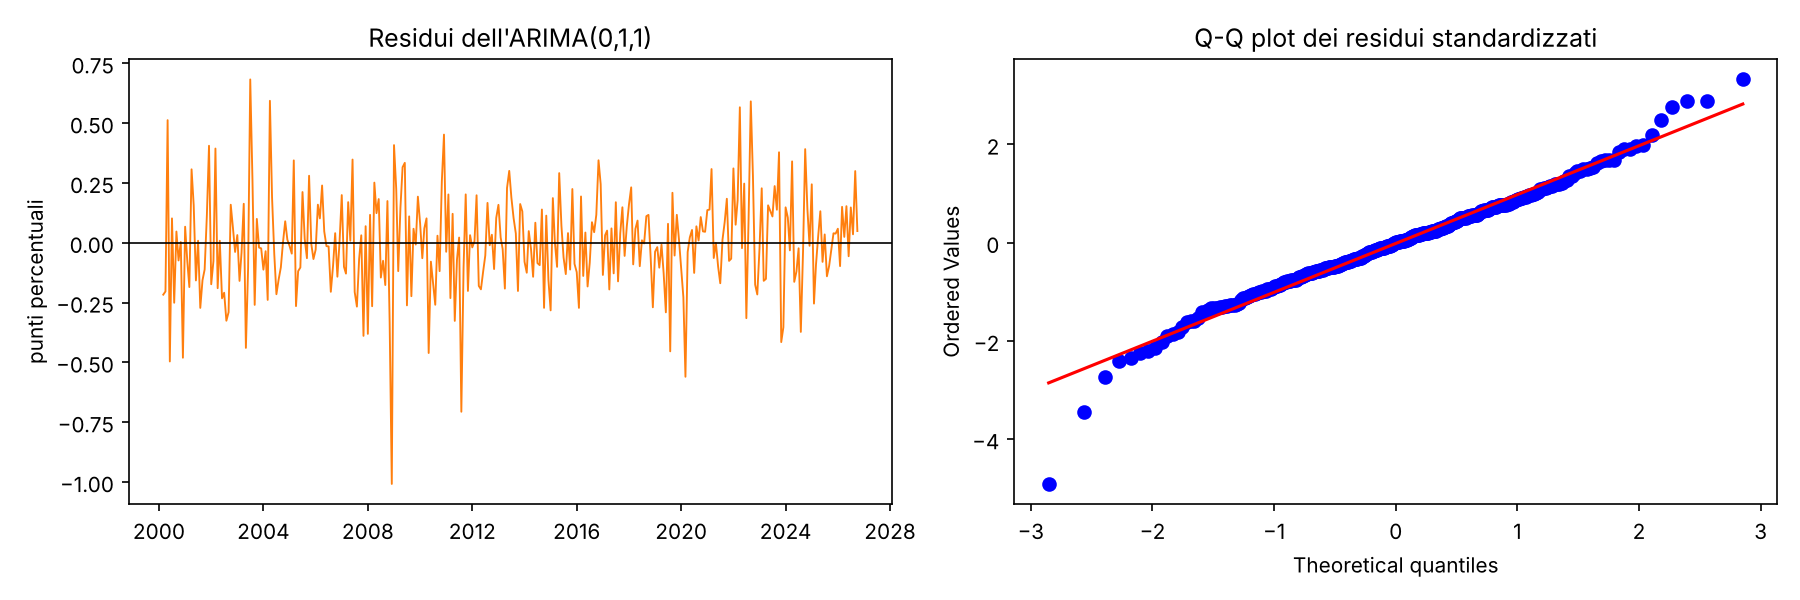
\includegraphics[width=0.92\textwidth]{figures/residui.png}\\
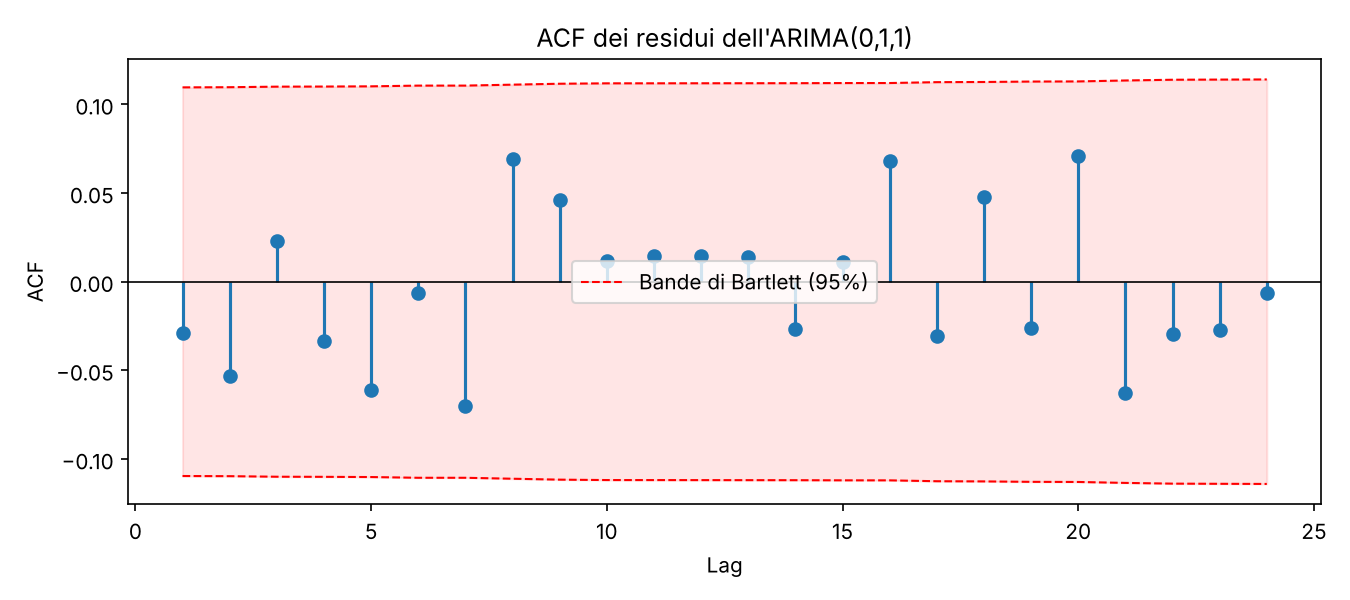
\includegraphics[width=0.62\textwidth]{figures/acf_residui.png}
\caption{Residui, Q-Q plot e ACF dei residui.}
\end{figure}

\begin{itemize}
\item \textbf{Autocorrelazione}: nessun rifiuto per $m = 6, 12, 24$, e nell'ACF dei residui nessuna barra supera $0{,}071$. Un solo parametro ha eliminato l'autocorrelazione presente in $\Delta y_t$ (il DW passa da $1{,}51$ a $2{,}05$).
\item \textbf{Normalità}: Jarque-Bera
\(
JB = \frac{T}{6}\left(S^2 + \frac{(K-3)^2}{4}\right) = 64{,}5
\)
con $S = -0{,}24$ e $K = 5{,}15$: normalità rifiutata per le code spesse (visibili alle estremità del Q-Q plot). Stime e previsioni puntuali restano valide; gli intervalli basati sulla normale vanno verificati fuori campione (sezione~\ref{sec:oos}).
\end{itemize}

\begin{nota}
\textbf{Perché non il Durbin-Watson.} Il DW (con $d_L$, $d_U$ tabulati) vale per regressioni senza dinamica stimata e la versione precedente usava le soglie per $T \approx 100$. Con un modello ARMA si usa il Ljung-Box: il DW è riportato solo come indicazione, $d \approx 2(1-\hat\rho_1)$.
\end{nota}

%=====================================================================
\section{Stabilità del parametro}

Il modello è stimato separatamente sulle due metà del campione e i coefficienti sono confrontati con $z = (\hat\theta_1 - \hat\theta_2)/\sqrt{SE_1^2 + SE_2^2}$.

\begin{table}[H]
\centering
\begin{tabular}{lcc}
\toprule
Sottocampione & $\hat\theta$ & SE \\
\midrule
2000-01 -- 2013-05 & $0{,}247$ & $0{,}096$ \\
2013-06 -- 2026-10 & $0{,}298$ & $0{,}099$ \\
\midrule
Differenza & $z = -0{,}37$ & p-value $0{,}71$ \\
\bottomrule
\end{tabular}
\end{table}

La differenza non è significativa: $\theta$ è \textbf{stabile} attraverso regimi molto diversi (crisi del 2008, tassi vicini allo zero, rialzo del 2022). È coerente con la spiegazione della sezione 4: l'MA(1) dipende dal modo in cui i dati sono costruiti (medie mensili), non dalla fase del ciclo.

%=====================================================================
\section{Valutazione fuori campione}\label{sec:oos}

Le ultime 64 osservazioni (da 2021-07, il 20\% del campione, che comprende il rialzo dei tassi del 2022) sono previste \textbf{a un passo con origine mobile}: per ogni mese il modello è ristimato su tutti i dati precedenti. Metriche:
\[
RMSE = \sqrt{\tfrac1n\textstyle\sum e_t^2}, \qquad MAE = \tfrac1n\textstyle\sum |e_t|,
\]
la \textbf{copertura} degli intervalli al 95\% (quota di dati veri dentro l'intervallo) e il test di \textbf{Diebold-Mariano},
\[
d_t = e_{1,t}^2 - e_{2,t}^2, \qquad DM = \frac{\bar d}{\sqrt{\hat\sigma^2_{LR}(d)/n}} \sim N(0,1),
\]
con $H_0$: stesso errore quadratico atteso ($DM < 0$: il modello 1 prevede meglio).

\begin{table}[H]
\centering
\begin{tabular}{lcccc}
\toprule
Modello & RMSE & MAE & Copertura 95\% & RMSE / RMSE RW \\
\midrule
\textbf{ARIMA(0, 1, 1)} & $\mathbf{0{,}2086}$ & $\mathbf{0{,}1616}$ & \textbf{95,3\%} & $\mathbf{0{,}938}$ \\
ARIMA(2, 1, 0) & $0{,}2087$ & $0{,}1610$ & 96,9\% & $0{,}938$ \\
ARIMA(1, 1, 1) & $0{,}2093$ & $0{,}1622$ & 95,3\% & $0{,}941$ \\
ARIMA(15, 1, 1) & $0{,}2188$ & $0{,}1676$ & 93,8\% & $0{,}984$ \\
Random walk & $0{,}2225$ & $0{,}1733$ & 93,8\% & $1{,}000$ \\
Random walk + drift & $0{,}2262$ & $0{,}1758$ & 92,2\% & $1{,}017$ \\
\bottomrule
\end{tabular}
\caption{Previsioni a un passo fuori campione (64 mesi).}
\end{table}

\begin{itemize}
\item L'ARIMA(0,\,1,\,1) ha l'RMSE più basso, circa il \textbf{6\% in meno del random walk}. Diebold-Mariano: $DM = -1{,}78$, p-value unilaterale $0{,}038$ (bilaterale $0{,}075$). Il guadagno è modesto, come ci si aspetta per un tasso di mercato, ma sistematico.
\item ARIMA(2,\,1,\,0) e ARIMA(1,\,1,\,1) prevedono quasi allo stesso modo: descrivono la stessa dinamica a un ritardo con un parametro in più.
\item L'ARIMA(15,\,1,\,1) prevede peggio dell'MA(1) ($DM = -1{,}93$, p-value unilaterale $0{,}027$): i parametri in eccesso adattano il rumore del campione (\textbf{sovradattamento}).
\item Aggiungere il drift peggiora il random walk, coerentemente con il drift non significativo.
\item La copertura dell'ARIMA(0,\,1,\,1) è 95,3\%: nonostante le code spesse, gli intervalli a un passo sono affidabili.
\end{itemize}

\begin{figure}[H]
\centering
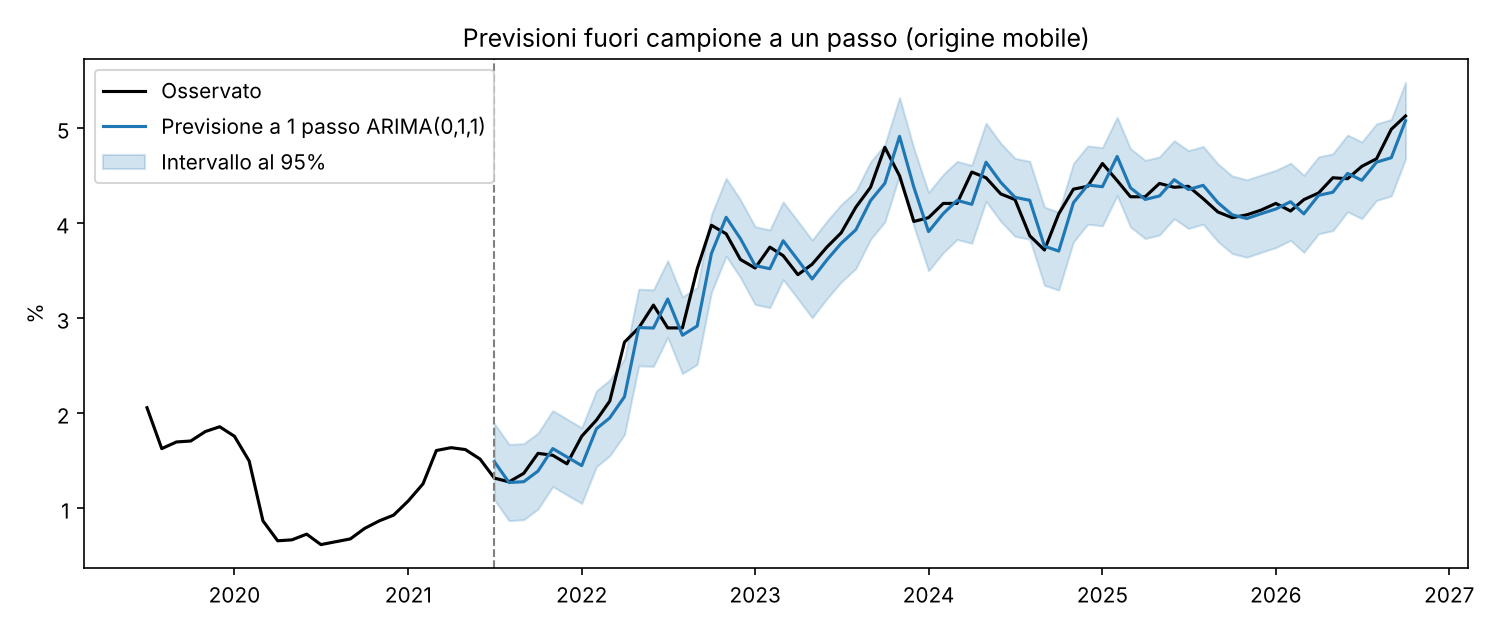
\includegraphics[width=0.9\textwidth]{figures/fuori_campione.png}
\caption{Previsioni a un passo fuori campione con intervallo al 95\%.}
\end{figure}

%=====================================================================
\section{Previsione a 12 mesi}

Con il modello stimato su tutti i dati, la previsione è ricorsiva: gli shock futuri sono posti a zero, quelli passati sostituiti dai residui. Per un ARIMA(0,\,1,\,1) senza drift:
\[
\hat y_{T+1} = y_T + \hat\theta\,\hat\varepsilon_T, \qquad \hat y_{T+h} = \hat y_{T+1} \ \ (h \ge 2).
\]
Sommando gli errori delle variazioni future, ogni shock $\varepsilon_{T+j}$ con $j < h$ pesa $1+\theta$ (una volta nel suo mese e $\theta$ volte nel successivo), tranne l'ultimo che pesa 1:
\[
Var(e_{T+h}) = \sigma^2\left[1 + (h-1)(1+\theta)^2\right],
\]
che cresce senza limite, come per ogni serie con radice unitaria.

\begin{table}[H]
\centering
\begin{tabular}{lcccc}
\toprule
Mese & $h$ & Previsione (\%) & SE & Intervallo al 95\% \\
\midrule
2026-11 & 1 & $5{,}145$ & $0{,}205$ & $[4{,}74;\ 5{,}55]$ \\
2026-12 & 2 & $5{,}145$ & $0{,}338$ & $[4{,}48;\ 5{,}81]$ \\
2027-01 & 3 & $5{,}145$ & $0{,}431$ & $[4{,}30;\ 5{,}99]$ \\
2027-04 & 6 & $5{,}145$ & $0{,}634$ & $[3{,}90;\ 6{,}39]$ \\
2027-10 & 12 & $5{,}145$ & $0{,}913$ & $[3{,}36;\ 6{,}93]$ \\
\bottomrule
\end{tabular}
\caption{Previsioni dal modello stimato su tutto il campione.}
\end{table}

\begin{figure}[H]
\centering
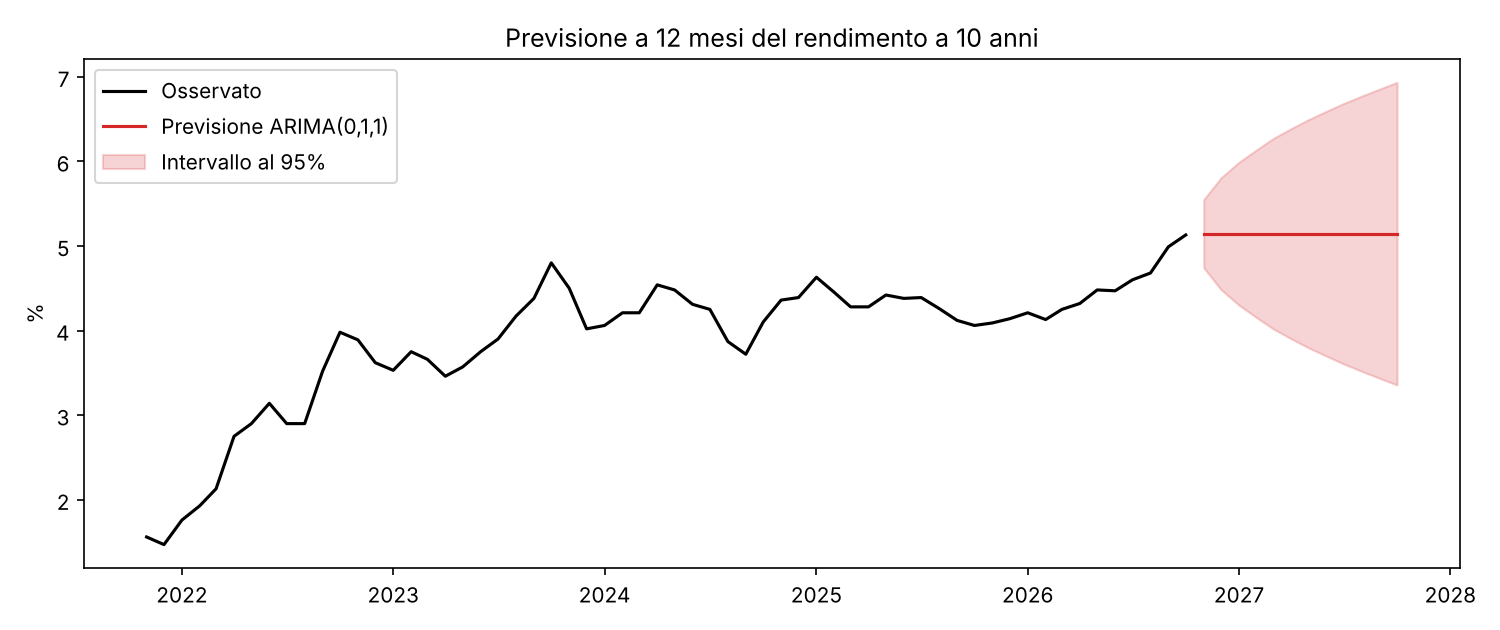
\includegraphics[width=0.85\textwidth]{figures/previsione.png}
\caption{Previsione a 12 mesi con intervallo al 95\%.}
\end{figure}

La previsione è di poco sopra l'ultimo dato (5{,}13\%), perché l'ultimo shock stimato è positivo ($\hat\varepsilon_T = 0{,}049$) e $\hat\theta$ ne trasmette una parte al mese successivo; poi resta piatta. A un anno l'intervallo al 95\% è largo circa $\pm1{,}8$ punti: con una radice unitaria e senza drift, quasi tutta l'informazione utile per prevedere il livello è nell'ultimo valore osservato.

%=====================================================================
\section{Verifica del codice}

\subsection{Errori trovati e correzioni}

\begin{center}
\small
\begin{tabular}{>{\raggedright\arraybackslash}p{3.2cm}>{\raggedright\arraybackslash}p{5.9cm}>{\raggedright\arraybackslash}p{5.5cm}}
\toprule
Dove & Problema & Correzione \\
\midrule
\texttt{LjungBox\_test} & \texttt{crit = chi2.cdf(q, dof)} è una probabilità, poi confrontata con $Q$: il test era sbagliato. & Valore critico $\chi^2_{dof,\,0.95}$ (\texttt{ppf}), p-value con \texttt{sf}; g.d.l.\ $m-p-q$ sui residui. \\
\texttt{JarqueBera\_test} & Usava la variabile globale \texttt{model}, \texttt{get\_stats} senza parentesi e chiavi inesistenti: errore all'esecuzione. & Lavora sui residui con \texttt{skewness}/\texttt{kurtosis} di \texttt{metrics.py}, p-value $\chi^2_2$. \\
\texttt{ARMA.train} & La parte MA era una regressione dei residui sui propri ritardi (un AR sui residui, non un MA); nessuna costante. & Hannan-Rissanen: AR lungo per stimare gli shock, poi OLS di $y_t$ su $y_{t-j}$ e $\tilde\varepsilon_{t-j}$. Aggiunti radici, pesi $\psi$, previsione, AIC/BIC. \\
Scelta di $p$, $q$ & Ultimo ritardo significativo su 20, e \texttt{max(.,1)}: $p = 15$ per caso e ordini forzati $\ge 1$. & Primo ritardo non significativo meno uno, poi selezione con AIC/BIC su campione comune. \\
\texttt{ACF\_test} & Bande $\pm1{,}96/\sqrt T$, valide solo sotto rumore bianco. & Bande di Bartlett. \\
\texttt{ADF\_test} & AIC confrontato su campioni diversi per ogni ritardo; solo versione \texttt{'ct'}; valore critico asintotico. & Campione comune per l'AIC, versioni \texttt{'c'}/\texttt{'ct'}, valori critici di MacKinnon per il $T$ effettivo. \\
\texttt{KPSS\_test} & Solo versione \texttt{'ct'}. & Aggiunta \texttt{'c'} (critico 0,463). \\
Notebook & Serie scelta con \texttt{adf\_ok or kpss\_ok} (basta uno dei due test); confronto ARMA/RW con varianze residue di serie diverse. & Decisione con entrambi i test più test sul drift; confronto fuori campione con RMSE e Diebold-Mariano. \\
\texttt{DW\_test} & Usato per accettare l'ARMA, con $d_L$, $d_U$ per $T\approx100$. & Sostituito dal Ljung-Box; DW solo indicativo. \\
Trasformazione & Logaritmo di un tasso trattato come prezzo. & Livelli (varianza più stabile, sezione 1). \\
\texttt{RandomWalk} & Calcolava la varianza di un coefficiente fissato a 1. & Drift opzionale, statistiche coerenti, previsione a $h$ passi. \\
\texttt{dataset.py} & Serie di default \texttt{"dataset"} invece di \texttt{"GS10"}; parametro \texttt{path} ignorato nel salvataggio. & Corretti. \\
\bottomrule
\end{tabular}
\end{center}

{\sloppy Aggiunti inoltre: \texttt{Trend\_test} (drift/trend con errori HAC), \texttt{T\_test}, \texttt{Coefficient\_test}, \texttt{Stability\_test}, \texttt{DieboldMariano\_test}, la classe \texttt{ARIMA}, la funzione \texttt{rolling\_one\_step} e le metriche \texttt{rmse}, \texttt{mae}, \texttt{coverage}, \texttt{aic}, \texttt{bic}, \texttt{long\_run\_variance}.\par}

\subsection{Confronto con \texttt{statsmodels}}

\begin{table}[H]
\centering
\begin{tabular}{lcc}
\toprule
Quantità & Progetto & \texttt{statsmodels} \\
\midrule
ADF 'ct' su y & $-1{,}4528$ & $-1{,}4528$ \\
ADF 'c' su $\Delta$y & $-12{,}3636$ & $-12{,}3636$ \\
KPSS 'ct' su y & $0{,}8619$ & $0{,}8619$ \\
KPSS 'c' su $\Delta$y & $0{,}4200$ & $0{,}4200$ \\
Ljung-Box $\Delta$y, m=12 & $27{,}4494$ & $27{,}4494$ \\
Jarque-Bera $\Delta$y & $83{,}1418$ & $83{,}1418$ \\
theta ARIMA(0,1,1) & $0{,}3053$ & $0{,}2950$ \\
SE theta & $0{,}0621$ & $0{,}0467$ \\
sigma & $0{,}2054$ & $0{,}2051$ \\
previsione h=1 & $5{,}1448$ & $5{,}1453$ \\
SE previsione h=12 & $0{,}9128$ & $0{,}9045$ \\
\bottomrule
\end{tabular}
\caption{Le statistiche dei test coincidono. Per l'ARIMA \texttt{statsmodels} usa la massima verosimiglianza esatta: $\hat\theta$ differisce di circa 0,01 e l'errore standard di Hannan-Rissanen è più grande (seconda regressione più corta, shock stimati).}
\end{table}

%=====================================================================
\section{Conclusioni}

\begin{enumerate}
\item \textbf{Trasformazione.} GS10 è un tasso, non un prezzo: le variazioni in punti percentuali hanno varianza molto più stabile di quelle logaritmiche, quindi si modellano i livelli.
\item \textbf{Stazionarietà.} ADF e KPSS concordano: livello con radice unitaria, variazioni stazionarie ($d = 1$), drift non significativo.
\item \textbf{Dinamica.} Le variazioni non sono rumore bianco; ACF, PACF, AIC e BIC indicano un MA(1). La media mensile di un random walk giornaliero genera esattamente un MA(1) con $\theta = 2-\sqrt3$, compatibile con $\hat\theta = 0{,}305$.
\item \textbf{Bontà.} $\theta$ significativo e stabile, modello invertibile, residui senza autocorrelazione; code spesse ma copertura fuori campione vicina al 95\%.
\item \textbf{Previsione.} L'ARIMA(0,\,1,\,1) batte il random walk di circa il 6\% in RMSE e il modello ARMA(15,\,1) sovradattato della versione precedente.
\end{enumerate}

\textbf{Limiti.} La varianza non è modellata (code spesse, periodi più volatili come il 2022): un modello GARCH sarebbe il passo successivo, fuori dal programma del corso. Il guadagno predittivo nasce dalla media mensile: su dati giornalieri il tasso sarebbe molto più vicino a un random walk puro.

\vspace{0.8em}
{\small\textbf{Riferimento.} H.~Working (1960), \emph{Note on the Correlation of First Differences of Averages in a Random Chain}, Econometrica 28(4), 916--918.}

\end{document}
